\let\negmedspace\undefined
\let\negthickspace\undefined
\documentclass[journal]{IEEEtran}
\usepackage[a5paper, margin=10mm, onecolumn]{geometry}
%\usepackage{lmodern} % Ensure lmodern is loaded for pdflatex
\usepackage{tfrupee} % Include tfrupee package

\setlength{\headheight}{1cm} % Set the height of the header box
\setlength{\headsep}{0mm}     % Set the distance between the header box and the top of the text

\usepackage{gvv-book}
\usepackage{gvv}
\usepackage{cite}
\usepackage{amsmath,amssymb,amsfonts,amsthm}
\usepackage{algorithmic}
\usepackage{graphicx}
\usepackage{textcomp}
\usepackage{xcolor}
\usepackage{txfonts}
\usepackage{listings}
\usepackage{enumitem}
\usepackage{mathtools}
\usepackage{gensymb}
\usepackage{comment}
\usepackage[breaklinks=true]{hyperref}
\usepackage{tkz-euclide} 
\usepackage{listings}
% \usepackage{gvv}                                        
\def\inputGnumericTable{}                                 
\usepackage[latin1]{inputenc}                                
\usepackage{color}                                            
\usepackage{array}                                            
\usepackage{longtable}                                       
\usepackage{calc}                                             
\usepackage{multirow}                                         
\usepackage{hhline}                                           
\usepackage{ifthen}                                           
\usepackage{lscape}
\usepackage{tabularx}
\usepackage{array}
\usepackage{float}
\usepackage{multicol}

% Marks the beginning of the document
\begin{document}
\bibliographystyle{IEEEtran}
\vspace{3cm}

\title{Matrix theory}
\author{ai24btech11035 - V.Preethika}
\maketitle
\bigskip
\newcommand{\createMat}[2]{\begin{pmatrix} #1 \\ #2 \end{pmatrix}}
\renewcommand{\thefigure}{\theenumi}
\renewcommand{\thetable}{\theenumi}

\textbf{Question:} Find the coordinates of a point A where AB is a diameter of the circle with center (3, -1) and the point B is (2, 6).\\
	    
\begin{table}[h!]
	\centering
  
    \begin{tabular}{ |c|c|c| }
        \hline
	    \textbf{Point} & \textbf{Value} & \textbf{Description}\\ 
        \hline
	    $\text{C}$ & $(3, -1)$ & $\text{Centre of the cicle}$ \\ 
        \hline
	    $\text{B}$ & $(2, 6)$ & $\text{Given point B}$ \\ 
        \hline
	    $\text{A}$ & $(x, y)$ & $\text{Coordinates of A}$ \\ 
        \hline
    \end{tabular}



	\caption{Variables Used}
	\label{tab1.5.16}
\end{table}
    \solution
	\begin{align}
    \vec{C} &= \frac{\vec{A}+\vec{B}}{2} \\
		&= \frac{\createMat{x}{y} + \createMat{2}{6}}{2} \\
             &= \left(\frac{x+2}{2}, \frac{y+6}{2}\right)
	\end{align}
	  
    
		Given the centre of the circle $\vec{C}$ is (3,-1),we can write
    
		\begin{align}
    \left( \frac{x + 2}{2}, \frac{y + 6}{2} \right) = (3, -1)
		\end{align}
    
    By solving this two equations we get:
    \begin{align}
	    x &= 4 \\
	    y &= -8
    \end{align}

    
    Therefore, the coordinates of point $\vec{A}$ are (4, -8).
    

\begin{figure}[ht]
   \centering
   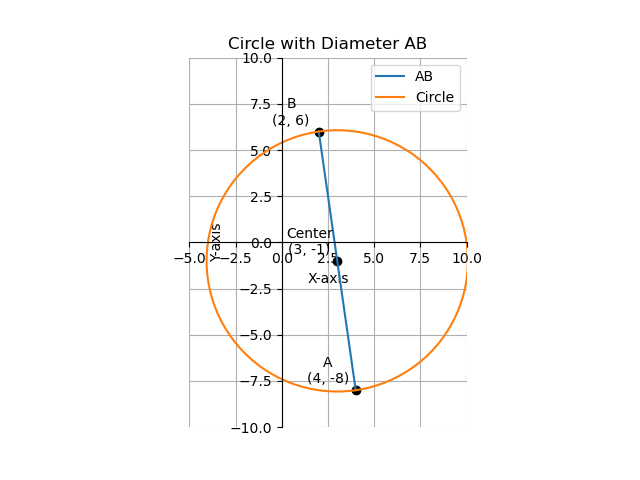
\includegraphics[width=0.7\linewidth]{Figs/circle.png}
   \caption{Graph of the Circle with Diameter AB}
   \label{q16}
\end{figure}

\end{document}

